%% Modelo de TCC - IFBA Euclides da Cunha
%% 
%% versao 1.0
%% 2024 Prof. Evilasio de Sousa Junior
%% https://github.com

%% Alteração do projeto bare_conf de Michael Shell
%% http://www.michaelshell.org/

%% Alteração do projeto Template para TCC na classe IFBATCC do Prof. Antônio Cleber de Sousa Araújo https://github.com/cleberaraujo/ifbatcc.git IFBA Santo Antõnio de Jesus

%%% Utiliza elementos do projeto ifbathesis.cls
%%%    Author              = "Luis Gustavo Cardoso Lima",
%%%    Version             = "1.0",
%%%    Date                = "21 Nov 2018",
%%%    Filename            = "ifbathesis.cls",
%%%    Address             = "Instituto Federal da Bahia
%%%                           GSORT",

%% Carrega a classe ifbatcc
%% Opcoes: * Idiomas
%%           pt   - português (padrao)
%%           en   - inglês
%%         * Tipos de Trabalhos (pelos graus de formação)
%%           tec  - para TCC de cursos tecnólogos (padrão)
%%           bsc  - para monografias de graduação
%%           msc  - para dissertações de mestrado
%%           qual - exame de qualificação de mestrado
%%           prop - exame de qualificação de doutorado
%%           phd  - para teses de doutorado
%%         * Cursos do IFBA/EUC
%%           ads  - Análise e Desenvolvimento de Sistemas
%%           rde  - Redes de Computadores (padrão)
%%           mul  - Produção Multimídia
%%         * Mídia
%%           scr  - para versão eletrônica (PDF) / consulte o guia do usuário
%%         * Estilo
%%           classic - estilo original a la TAOCP (deprecated)
%%           std     - novo estilo a la CUP (padrão)
%%         * Paginação
%%           oneside - para impressão em face única
%%           twoside - para impressão em frente e verso (padrão)
\documentclass[tec, rde, classic, a4paper]{arq_base/x_cuidado_com_esse_arquivo}
\usepackage[utf8]{inputenc}
\usepackage[printonlyused, withpage]{acronym}

%% Preâmbulo:
%% coloque aqui o seu preambulo LaTeX, i.e., declaração de pacotes,
%% (re)definicoes de macros, medidas, etc.

%% VARIÁVEIS

\author{NOME DO/DA AUTOR/A 1 \\ NOME DO/DA AUTOR/A 2 }
\title{TITULO DO TRABALHO}
\adviser{Nome do(a) Orientador(a)}
\texttype{Trabalho de Conclusão de Curso }
%\coadviser{Nome do/da Orientador/a}
% \course{rde}
%% Inicio do documento
\begin{document}


    \ifbacapa %% Capa do TCC
    \clearpage
    \ifbacontracapa{} %%Apresentação do Trabalho


    %% Termo de aprovação
    %% Composição da Banca Avaliadora
    \approvalsheet{Data da Aprovação, XX / XX / XXXX}{
      \comittemember{Profa. Dra. Nome da Professora 1}{Instituto Federal da Bahia}
      \comittemember{Prof. Me. Nome do Professor 2}{Instituto Federal da Bahia}
      \comittemember{Profa. Me. Nome da Professora 3}{Instituto Federal da Bahia}
    }


    \clearpage

    % Dedicatória
    % Comente para ocultar
    \begin{dedicatory}
    DIGITE A DEDICATÓRIA AQUI
    \end{dedicatory}
    
    % Agradecimentos
    % Se preferir, crie um arquivo a parte e o inclua via \include{}
    \agradecimentos{
        Digite os agradecimentos aqui
    }
    
    
    % Epigrafe
    % Comente para ocultar
    % e.g.
    %  \begin{epigraph}[Tarde, 1919]{Olavo Bilac}
    %  última flor do Lácio, inculta e bela,\\
    %  És, a um tempo, esplendor e sepultura;\\
    %  Ouro nativo, que, na ganga impura,\\
    %  A bruta mina entre os cascalhos vela.
    %  \end{epigraph}

    \clearpage
    
    \begin{epigraph}[NOTA]{AUTOR}
    DIGITE AQUI A CITACAO
    \end{epigraph}


    
\chapter*{\resumoname}
\thispagestyle{empty}
% Resumo em Portugues
Apresentar de forma sucinta e conectada, cada um dos itens a seguir: Contexto. Motivação. Problema. Justificativa. Objetivos/Proposta de Solução e  Resultados.

\par\vskip\baselineskip\noindent{\bf\textbf{Palavras-chave}: De, três a cinco, palavras-chave, Aqui. }


    
    \listoffigures % Lista de figuras %Gerado Automáticamente
\thispagestyle{empty} % Gerado Automaticamente
    \listoftables % Lista de tabelas %Gerado Automáticamente
\thispagestyle{empty} % Gerado Automaticamente
    
    %%%%%%%%%%%%%%%%%%%%%%%%%%%%%%%%%%%%%%%%%%%%%%%%%%%%%%
% Sintaxe da lista de acordo com a documentação do pacote `acronym'
% documentação: http://mirror.unl.edu/ctan/macros/latex/contrib/acronym/acronym.pdf
\chapter*{LISTA DE ABREVIATURAS E SIGLAS}
\begin{acronym}[]
    \acro{IHC}{Interface Humano-Computador}
    
\end{acronym}
%%%%%%%%%%%%%%%%%%%%%%%%%%%%%%%%%%%%%%%%%%%%%%%%%%%%%%
\thispagestyle{empty}
    
    \tableofcontents % Sumario % Gerado Automáticamente

    
                                    \mainmatter %% Parte textual
    
    %%%%%%%%%%%%%%%%%%%%%%%%%%%%%%%%%%%%%%%%%%%%%%%%%%%%%%
\xchapter{Introdução}{Um breve resumo deste capítulo}
\label{cap:introducao}
%%%%%%%%%%%%%%%%%%%%%%%%%%%%%%%%%%%%%%%%%%%%%%%%%%%%%%




\section{Contexto e Motivação} \textbf{ }
% descrição da situação, ambiente e circunstâncias em que o problema ou questão de pesquisa ocorre. 


\section{Problema e Justificativa}\textbf{ }



\section{Objetivos} \textbf{ } 
%Proposta de Solução de Software / Hardware / Tecnologias


\section{Resultados Esperados} \label{metodo} \textbf{ }
% Software deesnvolvido
% Código fonte publicado 
% Implantação da Solução para testes


\section{Organização do Texto}\textbf{ }
Além desta Introdução, este trabalho está organizado da seguinte forma: 

 \begin{itemize}
   \item O Capítulo \ref{cap:revisao} apresenta a revisão bibliográfica e a pesquisa sobre trabalhos relacionados;
   
   \item O Capítulo \ref{cap:desenvolvimento} descreve o planejamento do desenvolvimento, o mapeamento das necessidades e as etapas do processo de construção da solução / software;
   
   \item O Capítulo \ref{cap:conclusao} traz os resultados, reúne as considerações finais e traz as contribuições para a comunidade / área.
   
 \end{itemize}
    
    %%%%%%%%%%%%%%%%%%%%%%%%%%%%%%%%%%%%%%%%%%%%%%%%%%%%%%
\xchapter{Revisão Bibliográfica}{Este capítulo traz a fundamentação teórica relacionada aos assuntos abordados ao longo do trabalho e foi dividida em ...}
\label{cap:revisao}
%%%%%%%%%%%%%%%%%%%%%%%%%%%%%%%%%%%%%%%%%%%%%%%%%%%%%%

\section{Fundamentação Teórica} \textbf{ }
% Deve conter os conceitos obtidos na literatura e mencionadas no desenvolvimento

    Esta seção traz conceitos relacionados às .... dados geográficos e estatísticos e ...
    
    \subsection{Dados Geográficos e Estatísticos} \textbf{ } \newline

        Lorem ipsum dolor sit amet, consectetur adipiscing elit. Praesent ac tellus turpis. Donec vitae lorem odio. Sed luctus vestibulum libero eget pellentesque. Vivamus in mi turpis. Donec molestie feugiat sollicitudin. Nam et eleifend tortor. Cras lacinia, magna in tristique consequat, urna lorem placerat odio, id viverra mi nulla nec sem. Ut imperdiet, felis a hendrerit imperdiet, velit metus eleifend diam, ut convallis neque augue vitae leo. Morbi condimentum rhoncus faucibus. Fusce elit justo, semper lobortis blandit sed, lacinia et ligula. Pellentesque elit magna, vestibulum vitae adipiscing in, tincidunt eu erat. Nullam eu lectus vel nunc eleifend consectetur. Phasellus faucibus blandit nisi, eget fermentum erat tincidunt et. Aliquam ullamcorper varius nunc, nec eleifend dolor porttitor eu. Etiam eget nunc eu erat facilisis consequat sed accumsan urna. Nam vitae eros et justo iaculis gravida in sed nisl. Donec auctor gravida ipsum. Morbi sed ipsum tortor, quis ornare purus.
        
    \subsection{Painéis de Visualização de Informação - \textit{Dashboards}} \textbf{ } 

        %Exemplo de Citação. \citeonline() Deve estar no biblio.bib
        O desenvolvimento de \textit{dashboards} e a visualização de dados são tratados por \citeonline{few2006information} na obra ``Criação de \textit{dashboards} informativos: A comunicação visual eficaz dos dados''. Nela foram definidos aspectos que devem ser observados para a construção de painéis de visualização e estes foram descritos a seguir:

        %Exemplo de Listagem por Símbolos
        \begin{itemize}
            \item Informações organizadas para apoiar seu significado e uso;
            \item Consistência mantida para uma interpretação rápida e precisa;
            \item Visualização esteticamente agradável;
            \item \textit{Design} para uso como plataforma de lançamento;
            \item Avaliação da Usabilidade nos painéis criados.
        \end{itemize}

        \textbf{ } \\
        
        %Exemplo de Enumeração
        Exemplo de Enumeração
        \begin{enumerate}
            \item Exemplo de Item 1;
            \item Exemplo de Item 2.
        \end{enumerate}

        \clearpage %Quebra de Página
        
        Para \citeonline{few2006information}, painéis de visualização devem ser projetados de acordo com aspectos importantes do design visual e de usabilidade:

        %Exemplo de Citação Longa 
        \begin{quoting}[rightmargin=0cm,leftmargin=4cm]
        \begin{singlespace}
        {\footnotesize    
            Alguns aspectos importantes do \textit{design} visual do painel ainda precisam ser considerados. Um dos mais desafiadores é a necessidade de organizar muitos itens de informação, muitas vezes relacionados apenas pela necessidade do espectador de monitorá-los todos de uma maneira que não resulte em uma bagunça desordenada. Este arranjo deve apoiar as relações intrínsecas entre os vários itens e a maneira pela qual eles devem ser navegados e utilizados para apoiar a tarefa em questão. O design de um painel deve suportar seu uso de forma otimizada e transparente. O todo também deve ser agradável de se ver, ou será ignorado 
            (\citeonline{few2006information}, p. 138).
        }
        \end{singlespace}
        \end{quoting}
        
        \citeonline{few2006information} afirma ainda que a usabilidade é um aspecto a ser observado, e avaliações de usabilidade na área de conhecimento da \acf{IHC}, tem em suas origens as propostas e diretrizes de \citeonline{nielsen1990heuristic}. 


\section{Trabalhos Relacionados} \label{sec:trabrelac} \textbf{ }

% trazer exemplos de outros trabalhos que fazem algo na linha do seu trabalho.
    Foram reunidas algumas pesquisas correlatas ao problema de pesquisa que se pretende investigar, particularmente estudos para análises visuais de ...

    \textbf{ } 

    \citeonline{santos2018plataforma} propõe uma plataforma distribuída de mineração de dados para \textit{Big Data} e realiza um estudo de caso com notas fiscais de consumidores, disponibilizados pela Secretaria de Tributação do Rio Grande do Norte. Os trabalhos se aproximam em alguns aspectos como a manipulação, processamento e extração de conhecimento a partir de grande volume de dados
    
    %%%%%%%%%%%%%%%%%%%%%%%%%%%%%%%%%%%%%%%%%%%%%%%%%%%%%%
\xchapter{Desenvolvimento}{Um breve resumo deste capítulo}
\label{cap:desenvolvimento}
%%%%%%%%%%%%%%%%%%%%%%%%%%%%%%%%%%%%%%%%%%%%%%%%%%%%%%


\section{Coleta e Análise de Dados} \label{analise} \textbf{ }
% Apresentar dados, gráficos e estudos de caso

    \citeonline{cohn2004user} descreve as seguintes técnicas para criação de um conjunto de histórias:
    \begin{itemize}
        \item Entrevistas com usuários;
        \item Questionários;
        \item Observação;
        \item Oficinas de redação de histórias.
    \end{itemize}

    Este trabalho utilizou-se de entrevistas com usuários reais para a construção do protótipo funcional.


\section{Implementação da Solução} \label{implement} \textbf{ }
% Apresentar o sistema neste capítulo

    \subsection{Apresentação do Software e das Tecnologias utilizadas} \textbf{ }

    \clearpage
    \subsection{Funcionalidades} \textbf{ }

        %Exemplo de tabela
        a Tabela \ref{tab:classification-of-gof-patterns} traz o detalhamento do ...
        
        \begin{table}[ht] 
        \caption{Classificação dos padrões de projeto GOF.}
        \label{tab:classification-of-gof-patterns}
        \begin{tabular*}{1\columnwidth}{@{\extracolsep{\fill}}>{\raggedright}p{0.25\columnwidth}>{\raggedright}p{0.75\columnwidth}}
        \toprule 
        \textbf{Element} & \textbf{Description}\tabularnewline
        \midrule
        \midrule 
        Patterns & Top element of the schema.\\It represents a collection of\\types of patterns\tabularnewline
        \midrule 
        Structurals & The set of Design Patterns classified as structural.\\Example: Decorator\\Design Pattern\tabularnewline
        \midrule 
        Behaviourals & The set of Design Patterns classified as creational.\\Example: Observer\\Design Pattern\tabularnewline
        \midrule 
        Creationals & The set of Design Patterns classified as behavioral.\\Example: Singleton\\Design Pattern\tabularnewline
        \midrule 
        \bottomrule
        \end{tabular*}
        \centering \\Fonte: Autores, 2024.
        \end{table}

            
    \clearpage
    
    \subsection{Imagens do Uso do Software} \textbf{ }

        % Exemplo de explicação de figura no texto
        A Figura \ref{fig:ifba-euc} mostra a imagem do Campus Euclides da Cunha.

        % Exemplo de inserção de figura no texto
        % A tabela de figura é atualizada automáticamente
        \begin{figure}[ht]
            \fontsize{12pt}{12pt}\selectfont
            \caption{IFBA - Campus Euclides da Cunha}
            \label{fig:ifba-euc}
            
            \centering
            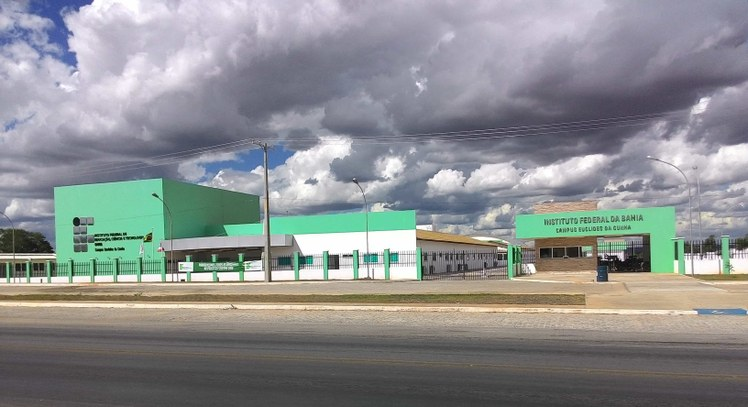
\includegraphics[scale=0.5]{imagens/ifba_euc.jpeg}
            \begingroup
                \fontsize{10pt}{10pt}\selectfont
                \centering \\Fonte: Autores, 2024.
            \endgroup
        \end{figure}  

        \clearpage
        Exemplo de algoritmo \ref{alg:BA}.
        \begin{algorithm}[ht]\label{alg:BA}
        \caption{\textit{Baseline Algorithm} (BA)}
        \small
        \KwIn{$Q=\{Q.D, Q.A, Q.T\}$}
        $R \leftarrow \emptyset$ \\
        \For{\textbf{each} $p \in P$}{ 
        	$containsAllTerms = \textit{true}$\\
        	\For{\textbf{each} $d \in Q.D$}{
        		$containsTerm = false$\\
        		\For{\textbf{each} $d' \in p.D$}{
        			\If{$d' = d$}{
        				$containsTerm = \textit{true}$
        			}
        		}
        		\If{\textbf{not} $containsTerms$}{
        			$containsAllTerms = false$
        		}
        	}
        	\If{$containsAllTerms$}{
        		\If{$Q.A_{1x} \leq p.x < Q.A_{2x}$ \textbf{and} $Q.A_{1y} \leq p.y \leq Q.A_{2y}$}{
        		\If{$Q.T_{1} \leq p.T \leq Q.T_{2}$}{
        			$R \leftarrow R \cup p$
        			}
        		}
        	}
        }
        \textbf{return} $R$
        \end{algorithm} 

    %%%%%%%%%%%%%%%%%%%%%%%%%%%%%%%%%%%%%%%%%%%%%%%%%%%%%%
\xchapter{Conclusão}{Um breve resumo deste capítulo}
\label{cap:conclusao}
%%%%%%%%%%%%%%%%%%%%%%%%%%%%%%%%%%%%%%%%%%%%%%%%%%%%%%
% Síntese das principais conclusões da pesquisa

\section{Considerações}
% Conclusão da Pesquisa

    O presente trabalho teve como objetivo construir e apresentar o \textbf{Nome do Software que foi desenvolvido}, solução capaz de oferecer ...

    \textbf{ }
    
    Apresentar se o software cumpriu o objetivo (Resultados)

\section{Limitações e Trabalhos Futuros} \textbf{ }

    Este trabalho limitou-se a tratar apenas com a ...

    \textbf{ }
    
    Sugere-se como proposta de trabalho futuro a realização de estudos sobre ...
    
                                    \backmatter  %% Parte pós-textual
    
    
    \bibliographystyle{abntex2-alf}
    \bibliography{05_biblio.bib} % Bibliografia BibTeX
    
\end{document}